\documentclass{article}

\usepackage{../../common}

\graphicspath{
  {../../../media/images/}
}
\addbibresource{../../references.bib}

\title{Rovinné geometrické útvary}

\begin{document}

\maketitle

\section{Rovinné geometrické útvary}

Rovinné geometrické útvary sú útvary, ktoré môžeme nakresliť na rovnej ploche, teda v jednej rovine. Sú to napríklad útvary ako trojuholník, štvorec, obdĺžnik, kružnica atď. Rovinné útvary majú dva rozmery: dĺžku a šírku. Na rozdiel priestorové útvary (kocka, guľa, valec) majú tri rozmery: dĺžku, šírku a výšku.

\subsection{Kružnica a kruh}

Kružnica je súbor bodov, ktoré majú rovnakú vzdialenosť od jedného pevného bodu nazývaného ako stred kružnice. Kružnicu označujeme malými písmenami abecedy \(k\), \(l\), \(m\)\dots Vzdialenosť stredu kružnice od ľubovoľného bodu sa nazýva polomer, označujeme \(r\). Priemer je dvojnásobok polomeru, označujeme \(d\). Kružnicu \(k\) so stredom \(S\) a polomerom \(r\) označujeme ako \(k(S, r)\). Každá kružnica je jednoznačne určená jej stredom a polomerom.

Kružnica je iba súbor bodov, ktorý tvorí oblúk, vnútro krúžnice je prázdne. Ak chceme zahrnúť aj vnútro, hovoríme o kruhu. Kruh je súbor bodov, ktoré majú menšiu alebo rovnakú vzdialenosť od jedného pevného bodu nazývaného ako stred kruhu. Kruh označujeme veľkými písmenami abecedy \(K\), \(L\), \(M\)\dots Polomer a priemer zachovávajú význam. Kruh \(K\) so stredom \(S\) a polomerom \(r\) označujeme ako \(K(S, r)\). Každý kruh je jednoznačne určený jeho stredom a polomerom.

Kružnica a kruh, spolu s priamkami a úsečkami, sú základné rovinné geometrické útvary. Pomocou nich dokážeme zostrojiť zložitejšie rovinné geometrické útvary, ako sú obdĺžniky, štvorce, päťuholníky atď.

\begin{center}
  \begin{minipage}{0.45\textwidth}
    \centering
    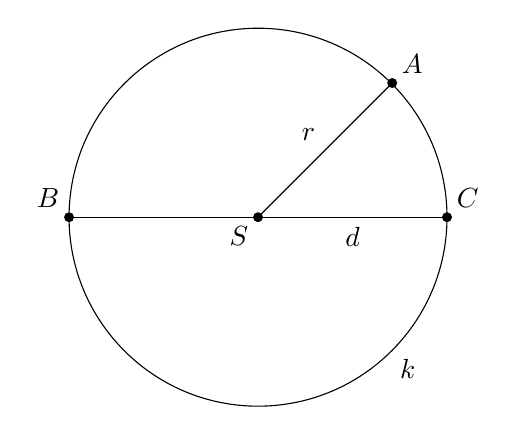
\begin{tikzpicture}[scale=1.2]
      \draw (0,0) circle (2cm);
      
      \fill (0,0) circle (1.5pt);
      \node[below left] at (0,0) {$S$};
      
      \draw (0,0) -- (1.42,1.42);
      \fill (1.42,1.42) circle (1.5pt);
      \node[above left] at (0.707,0.707) {$r$};
      \node[above right] at (1.42,1.42) {$A$};
      
      \draw (-2,0) -- (2,0);
      \fill (2,0) circle (1.5pt);
      \fill (-2,0) circle (1.5pt);
      \node[below] at (1,0) {$d$};
      \node[above left] at (-2,0) {$B$};
      \node[above right] at (2,0) {$C$};
      
      \node[below right] at (1.4,-1.4) {$k$};
    \end{tikzpicture}
    \[
      \begin{aligned}
      \text{kružnica}\ & k(S, r) \\
      \text{polomer kružnice}\ & r = |SA| \\
      \text{priemer kružnice}\ & d = |BC| = 2r
      \end{aligned}
    \]
  \end{minipage}
  \begin{minipage}{0.45\textwidth}
    \centering
    \begin{tikzpicture}[scale=1.2]
      \filldraw[
          pattern=north east lines,
          pattern color=red!40
      ] (0,0) circle (2cm);
      
      \fill (0,0) circle (1.5pt);
      \node[below left] at (0,0) {$S$};
      
      \draw (0,0) -- (1.42,1.42);
      \fill (1.42,1.42) circle (1.5pt);
      \node[above left] at (0.707,0.707) {$r$};
      \node[above right] at (1.42,1.42) {$A$};
      
      \draw (-2,0) -- (2,0);
      \fill (2,0) circle (1.5pt);
      \fill (-2,0) circle (1.5pt);
      \node[below] at (1,0) {$d$};
      \node[above left] at (-2,0) {$B$};
      \node[above right] at (2,0) {$C$};
      
      \node[below right] at (1.4,-1.4) {$k$};
    \end{tikzpicture}
    \[
      \begin{aligned}
      \text{kruh}\ & K(S, r) \\
      \text{polomer kruhu}\ & r = |SA| \\
      \text{priemer kruhu}\ & d = |BC| = 2r
      \end{aligned}
    \]
  \end{minipage}
\end{center}

\subsubsection{Konštrukcia kružnice a kruhu}

\begin{enumerate}[label=\arabic*)]
  \item Na kružidlo nanesieme dĺžku polomeru kružnice \(r\).
  \item Kružidlo zapichneme ostrým koncom do bodu \(S\).
  \item Kružidlom zostrojíme kružnicu \(k\) s polomerom \(r\).
\end{enumerate}

\subsection{Trojuholník}

Trojuholník je rovinný geometrický útvar, ktorý je ohraničený tromi úsečkami. Trojuholník má tri vrcholy a tri strany. Trojuholník označujeme tromi veľkými písmenami podľa jeho vrcholov, napríklad \(ABC\). Tri rôzne body, ktoré neležia na tej istej priamke, jednoznačne určujú trojuholník. Oproti vrcholom ležia ich strany, ktoré označujeme malými písmenami rovnakej hlásky. V trojuholníku \(ABC\) je oproti vrcholu \(A\) strana \(a\), oproti vrcholu \(B\) strana \(b\) a oproti vrcholu \(C\) strana \(c\).

V každom trojuholníku platí \emph{trojuholníková nerovnosť}. Súčet dĺžok ľubovoľných dvoch strán trojuholníka je vždy väčší ako dĺžka jeho tretej strany. Pre trojuholník \(ABC\) so stranami dĺžkami strán \(a\), \(b\), \(c\) platia nerovnosti:
\[
\begin{aligned}
  a + b &> c, \\
  a + c &> b, \\
  b + c &> a.
\end{aligned}
\]

\subsubsection{Konštrukcia trojuholníka}

Trojuholník môžeme narysovať vtedy, keď poznáme dĺžky všetkých jeho strán.

\begin{enumerate}[label=\arabic*)]
  \item Narysujeme úsečku \(AB\) dĺžky strany \(c\).
  \item Narysujeme kružnicu \(k_1\) so stredom v bode \(A\) a polomerom dĺžky strany \(b\).
  \item Narysujeme kružnicu \(k_2\) so stredom v bode \(B\) a polomerom dĺžky strany \(a\).
  \item Priesečník dvoch kružníc \(k_1\) a \(k_2\) je bod \(C\).
  \item Narysujeme úsečky \(AC\) a \(BC\).
  \item Zostrojili sme trojuholník \(ABC\).
\end{enumerate}

\subsection{Štvoruholníky}

Štvoruholník je rovinný geometrický útvar, ktorý je ohraničený štyrmi úsečkami. Štvoruholník má štyri vrcholy a štyri strany. Štvoruholníky označujeme štyrmi veľkými písmenami podľa jeho vrcholov, napríklad \(ABCD\). Vrcholy zapisujeme v poradí, ako idú za sebou po obvode štvoruholníka, teda štvoruholník \(ABCD\) má strany \(AB\), \(BC\), \(CD\) a \(DA\).

\end{document}